\subsection{Architectures and Training}
\label{sec:training}

\begin{figure}[tp]
    \vspace*{-\figskipabove px}
    \vspace{4px}
    \centering
    {\scriptsize
        
    \begin{subfigure}[t]{0.5\textwidth}
        \vspace{0px}\centering
	    \begin{subfigure}[t]{0.15\textwidth}
   	    	\vspace{0px}\centering
   	    	GT,\\High\\
	        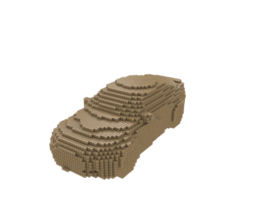
\includegraphics[width=1.5cm,trim={\cropleft cm \croplower cm \cropright cm \cropupper cm},clip]{gdat_shapenet_clean_high_0_bin_only}
	    \end{subfigure}
	    \begin{subfigure}[t]{0.15\textwidth}
   	    	\vspace{0px}\centering
   	    	GT\\
   	    	~\\
	        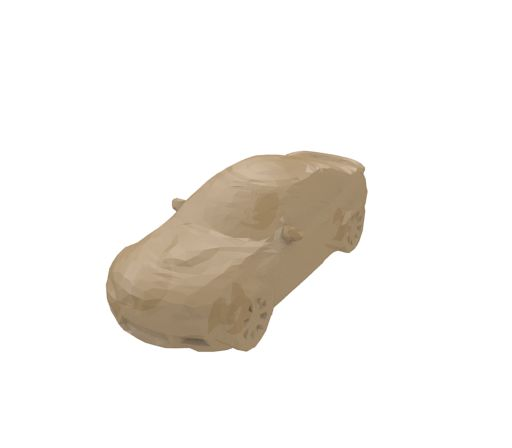
\includegraphics[width=1.5cm,trim={\cropleft cm \croplower cm \cropright cm \cropupper cm},clip]{gdat_shapenet_clean_low_0_gt_only}
	    \end{subfigure}
	    \begin{subfigure}[t]{0.15\textwidth}
   	    	\vspace{0px}\centering
   	    	\DVAE, Low\\
	        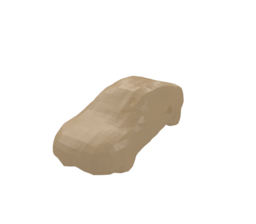
\includegraphics[width=1.5cm,trim={\cropleft cm \croplower cm \cropright cm \cropupper cm},clip]{gexp_clean_low_10_wide_prior_3_2_res_0}
	    \end{subfigure}
	    \begin{subfigure}[t]{0.15\textwidth}
   	    	\vspace{0px}\centering
   	    	\DVAE, High\\
   	    	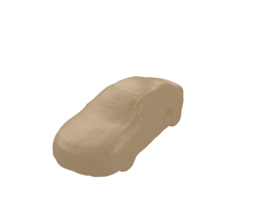
\includegraphics[width=1.5cm,trim={\cropleft cm \croplower cm \cropright cm \cropupper cm},clip]{gexp_clean_high_10_wide_prior_3_2_res_0}
	    \end{subfigure}
	    \begin{subfigure}[t]{0.15\textwidth}
   	    	\vspace{0px}\centering
   	    	\DVAE, Low\\
	        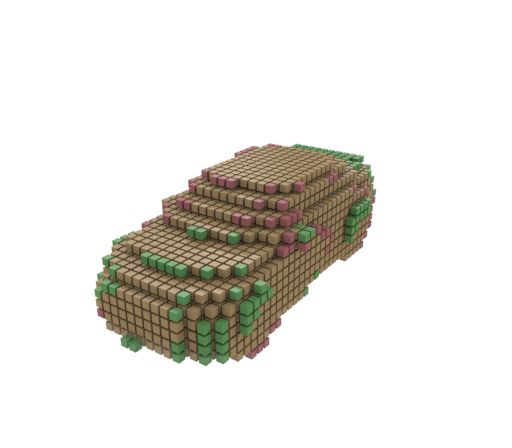
\includegraphics[width=1.5cm,trim={\cropleft cm \croplower cm \cropright cm \cropupper cm},clip]{gexp_clean_low_10_wide_prior_3_3_res_0}
	    \end{subfigure}
	    \begin{subfigure}[t]{0.15\textwidth}
   	    	\vspace{0px}\centering
   	    	\DVAE, High\\
	        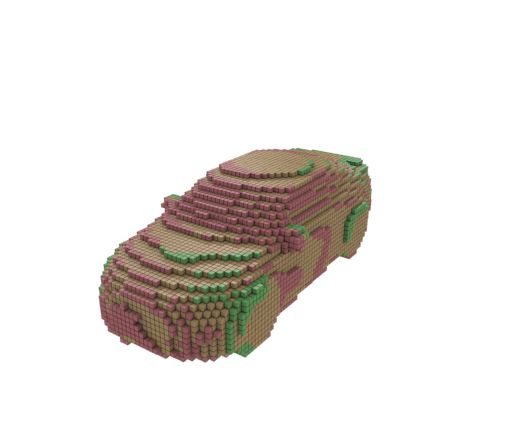
\includegraphics[width=1.5cm,trim={\cropleft cm \croplower cm \cropright cm \cropupper cm},clip]{gexp_clean_high_10_wide_prior_3_3_res_0}
	    \end{subfigure}
	    \\ %[-4px]
	    %\begin{subfigure}[t]{0.105\textwidth}
	    %	\vspace{0px}\centering
	    %	\includegraphics[width=1.5cm,trim={\cropleft cm \croplower cm \cropright cm \cropupper cm},clip]{gdat_modelnet_chair_low_1188_bin_only}
	    %\end{subfigure}
	    \begin{subfigure}[t]{0.15\textwidth}
   	    	\vspace{0px}\centering
	        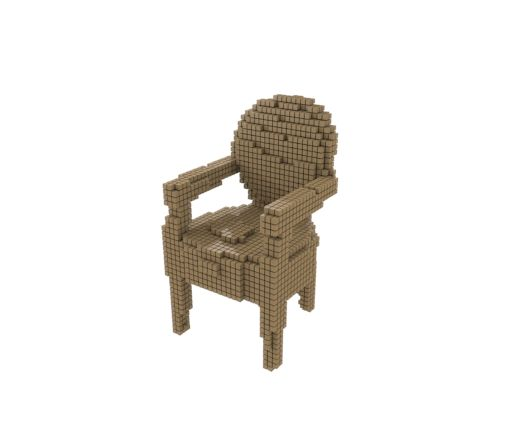
\includegraphics[width=1.5cm,trim={\cropleft cm \croplower cm \cropright cm \cropupper cm},clip]{gdat_modelnet_chair_high_1188_bin_only}
	    \end{subfigure}
	    \begin{subfigure}[t]{0.15\textwidth}
   	    	\vspace{0px}\centering
	        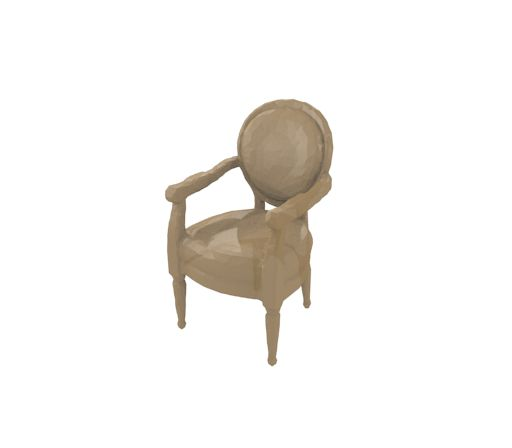
\includegraphics[width=1.5cm,trim={\cropleft cm \croplower cm \cropright cm \cropupper cm},clip]{gdat_modelnet_chair_low_1188_gt_only}
	    \end{subfigure}
	    \begin{subfigure}[t]{0.15\textwidth}
   	    	\vspace{0px}\centering
	        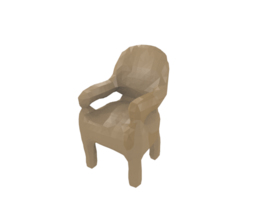
\includegraphics[width=1.5cm,trim={\cropleft cm \croplower cm \cropright cm \cropupper cm},clip]{gexp_clean_chair_low_10_wide_prior_3_2_res_1188}
	    \end{subfigure}
	    \begin{subfigure}[t]{0.15\textwidth}
   	    	\vspace{0px}\centering
   	    	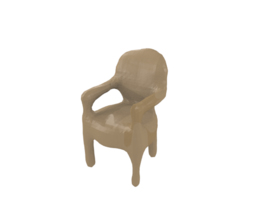
\includegraphics[width=1.5cm,trim={\cropleft cm \croplower cm \cropright cm \cropupper cm},clip]{gexp_clean_chair_high_10_wide_d_prior_3_2_res_1188}
	    \end{subfigure}
	    \begin{subfigure}[t]{0.15\textwidth}
   	    	\vspace{0px}\centering
	        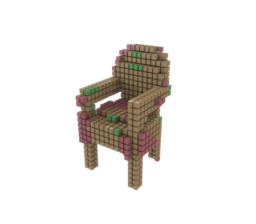
\includegraphics[width=1.5cm,trim={\cropleft cm \croplower cm \cropright cm \cropupper cm},clip]{gexp_clean_chair_low_10_wide_prior_3_3_res_1188}
	    \end{subfigure}
	    \begin{subfigure}[t]{0.15\textwidth}
   	    	\vspace{0px}\centering
	        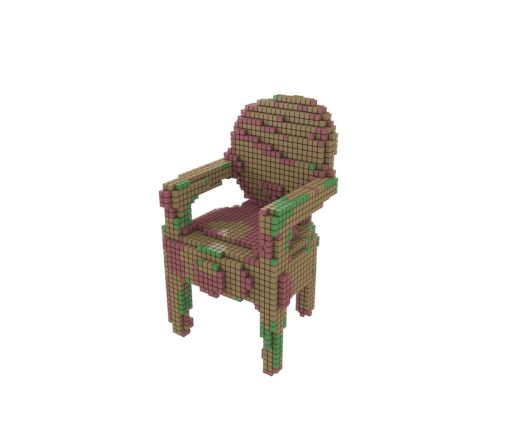
\includegraphics[width=1.5cm,trim={\cropleft cm \croplower cm \cropright cm \cropupper cm},clip]{gexp_clean_chair_high_10_wide_d_prior_3_3_res_1188}
	    \end{subfigure}
        \subcaption{Reconstructions, Low and High Resolution (\cf \tabref{tab:data})}
    \end{subfigure}
    \\[4px]
    \begin{subfigure}[t]{0.5\textwidth}
        \vspace{0px}\centering
	    \begin{subfigure}[t]{0.15\textwidth}
   	    	\vspace{0px}\centering
            Low\\
	        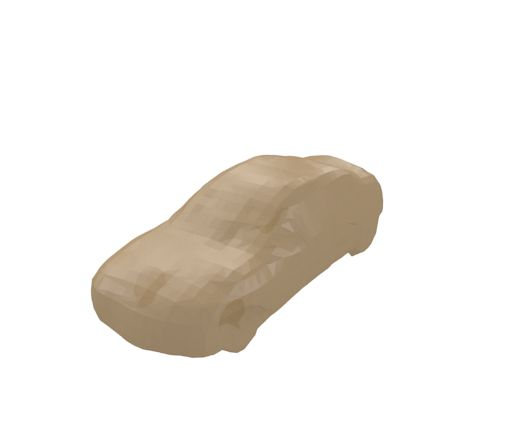
\includegraphics[width=1.5cm,trim={\cropleft cm \croplower cm \cropright cm \cropupper cm},clip]{gexp_clean_low_10_wide_prior_3_2_random_results_0}
	    \end{subfigure}
	    \begin{subfigure}[t]{0.15\textwidth}
   	    	\vspace{0px}\centering
            Low\\
	        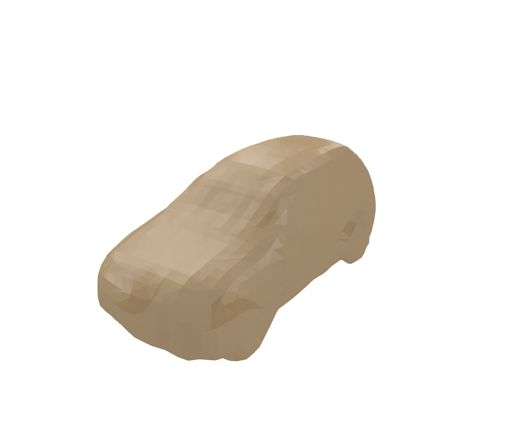
\includegraphics[width=1.5cm,trim={\cropleft cm \croplower cm \cropright cm \cropupper cm},clip]{gexp_clean_low_10_wide_prior_3_2_random_results_6}
	    \end{subfigure}
	    \begin{subfigure}[t]{0.15\textwidth}
   	    	\vspace{0px}\centering
            Low\\
	        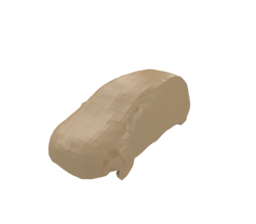
\includegraphics[width=1.5cm,trim={\cropleft cm \croplower cm \cropright cm \cropupper cm},clip]{gexp_clean_low_10_wide_prior_3_2_random_results_2}
	    \end{subfigure}
	    \begin{subfigure}[t]{0.15\textwidth}
   	    	\vspace{0px}\centering
            High\\
	        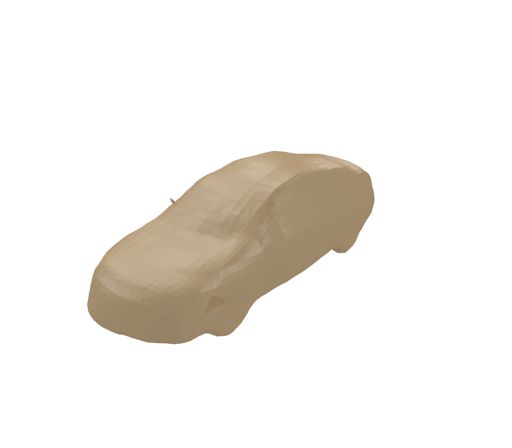
\includegraphics[width=1.5cm,trim={\cropleft cm \croplower cm \cropright cm \cropupper cm},clip]{gexp_clean_high_10_wide_prior_3_2_random_results_1}
	    \end{subfigure}
	    \begin{subfigure}[t]{0.15\textwidth}
   	    	\vspace{0px}\centering
            High\\
	        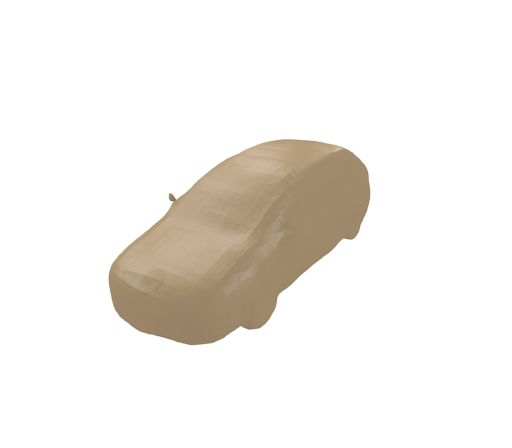
\includegraphics[width=1.5cm,trim={\cropleft cm \croplower cm \cropright cm \cropupper cm},clip]{gexp_clean_high_10_wide_prior_3_2_random_results_5}
	    \end{subfigure}
	    \begin{subfigure}[t]{0.15\textwidth}
   	    	\vspace{0px}\centering
            High\\
	        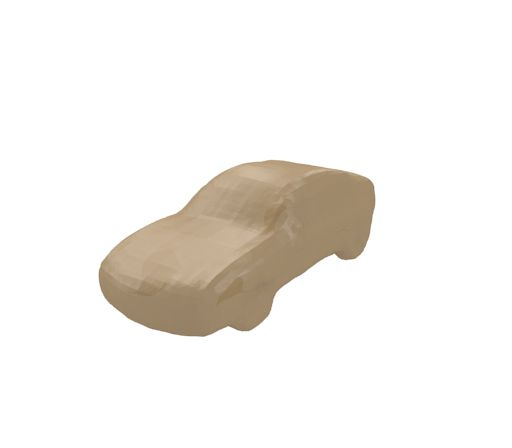
\includegraphics[width=1.5cm,trim={\cropleft cm \croplower cm \cropright cm \cropupper cm},clip]{gexp_clean_high_10_wide_prior_3_2_random_results_2}
	    \end{subfigure}
	    \\ %[-4px]
	    \begin{subfigure}[t]{0.15\textwidth}
   	    	\vspace{0px}\centering
   	       	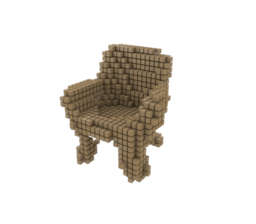
\includegraphics[width=1.5cm,trim={\cropleft cm \croplower cm \cropright cm \cropupper cm},clip]{gexp_clean_chair_low_10_wide_prior_3_3_random_results_1}
	    \end{subfigure}
	    \begin{subfigure}[t]{0.15\textwidth}
   	    	\vspace{0px}\centering
   	       	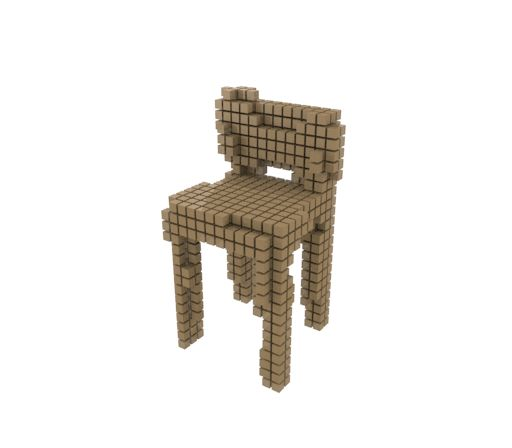
\includegraphics[width=1.5cm,trim={\cropleft cm \croplower cm \cropright cm \cropupper cm},clip]{gexp_clean_chair_low_10_wide_prior_3_3_random_results_6}
	    \end{subfigure}
	    \begin{subfigure}[t]{0.15\textwidth}
   	    	\vspace{0px}\centering
   	       	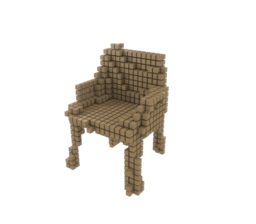
\includegraphics[width=1.5cm,trim={\cropleft cm \croplower cm \cropright cm \cropupper cm},clip]{gexp_clean_chair_low_10_wide_prior_3_3_random_results_2}
	    \end{subfigure}
	    \begin{subfigure}[t]{0.15\textwidth}
   	    	\vspace{0px}\centering
   	       	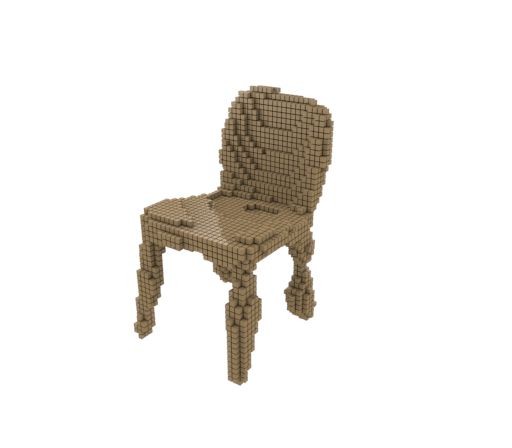
\includegraphics[width=1.5cm,trim={\cropleft cm \croplower cm \cropright cm \cropupper cm},clip]{gexp_clean_chair_high_10_wide_d_prior_3_3_random_results_1}
	    \end{subfigure}
	    \begin{subfigure}[t]{0.15\textwidth}
   	    	\vspace{0px}\centering
   	       	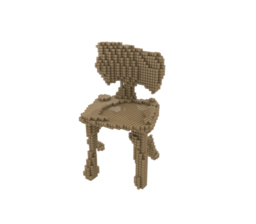
\includegraphics[width=1.5cm,trim={\cropleft cm \croplower cm \cropright cm \cropupper cm},clip]{gexp_clean_chair_high_10_wide_d_prior_3_3_random_results_0}
	    \end{subfigure}
	    \begin{subfigure}[t]{0.15\textwidth}
   	    	\vspace{0px}\centering
   	       	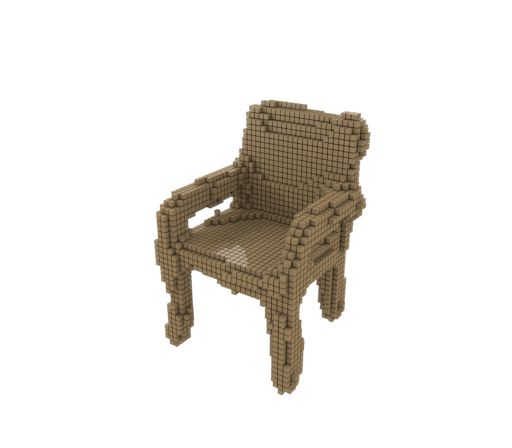
\includegraphics[width=1.5cm,trim={\cropleft cm \croplower cm \cropright cm \cropupper cm},clip]{gexp_clean_chair_high_10_wide_d_prior_3_3_random_results_3}
	    \end{subfigure}
        \subcaption{Random Samples, Low and High Resolution (\cf \tabref{tab:data})}
    \end{subfigure}
    }

    \vspace*{-\figskipcaption px}
    \caption{{\bf \DVAE Shape Prior.} Reconstructions and random samples on ShapeNet and ModelNet at multiple resolutions (\cf \tabref{tab:data}); false negative and false positive voxels in {\color{rgreen}green} and {\color{rred}red}. Our \DVAE shape prior provides high-quality reconstructions and meaningful random samples across resolutions.}
    \label{fig:results-shape-prior}
    \vspace*{-\figskipbelow px}
\end{figure}

As depicted in \figref{fig:architectures}, our network architectures are kept simple and shallow. Considering a resolution of $24 \ntimes 54 \ntimes 24$ voxels on ShapeNet and KITTI, the encoder comprises three stages, each consisting of two convolutional layers (followed by $\text{ReLU}$ activations and batch normalization \citep{Ioffe2015ICML}) and max pooling; the decoder mirrors the encoder, replacing max pooling by nearest neighbor upsampling. We consistently use $3^3$ convolutional kernels. We use a latent space of size $Q = 10$ and predict occupancy using Sigmoid activations.

We found that the shape representation has a significant impact on training. Specifically, learning both occupancy grids and SDFs works better compared to training on SDFs only. Additionally, following prior art in single image depth prediction \citep{Eigen2015ICCV,Eigen2014NIPS,Laina2016THREEDV}, we consider log-transformed, truncated SDFs (logTSDFs) for training: given a signed distance $y_i$, we compute $\text{sign}(y_i)\log(1 + \min(5, |y_i|))$ as the corresponding log-transformed, truncated signed distance. TSDFs are commonly used in the literature \citep{Newcombe2011ISMAR,Riegler2017THREEDV,Dai2017CVPRa,Engelmann2016GCPR,Curless1996SIGGRAPH} and the logarithmic transformation additionally increases the relative importance of values around the surfaces (\ie, around the zero crossing).

\begin{figure}[tp]
    \vspace*{-\figskipabove px}
    \vspace{4px}
    \centering
    {\scriptsize
        
    \newcommand{\ablationa}{33}
    \newcommand{\ablationb}{99}
    \newcommand{\ablationc}{528}
    \newcommand{\ablationd}{693}
    \newcommand{\ablatione}{231}
    \newcommand{\ablationf}{396} % 396
    
    \begin{subfigure}[t]{0.01\textwidth}
        \vspace{0px}\centering
        \rotatebox[]{90}{\dAML\hspace*{0.25cm}}
    \end{subfigure}
    \begin{subfigure}[t]{0.07\textwidth}
        \vspace{0px}\centering
        \includegraphics[width=1.5cm,trim={\cropleft cm \croplower cm \cropright cm \cropupper cm},clip]{gexp_noisy_low_10_wide_w2_1_aml_3_2_res_\ablationa}
    \end{subfigure}
    \begin{subfigure}[t]{0.07\textwidth}
        \vspace{0px}\centering
        \includegraphics[width=1.5cm,trim={\cropleft cm \croplower cm \cropright cm \cropupper cm},clip]{gexp_noisy_low_10_wide_w2_1_aml_3_2_res_\ablationb}
    \end{subfigure}
    \begin{subfigure}[t]{0.07\textwidth}
        \vspace{0px}\centering
        \includegraphics[width=1.5cm,trim={\cropleft cm \croplower cm \cropright cm \cropupper cm},clip]{gexp_noisy_low_10_wide_w2_1_aml_3_2_res_\ablationc}
    \end{subfigure}
    \begin{subfigure}[t]{0.07\textwidth}
        \vspace{0px}\centering
        \includegraphics[width=1.5cm,trim={\cropleft cm \croplower cm \cropright cm \cropupper cm},clip]{gexp_noisy_low_10_wide_w2_1_aml_3_2_res_\ablationd}
    \end{subfigure}
    \begin{subfigure}[t]{0.07\textwidth}
        \vspace{0px}\centering
        \includegraphics[width=1.5cm,trim={\cropleft cm \croplower cm \cropright cm \cropupper cm},clip]{gexp_noisy_low_10_wide_w2_1_aml_3_2_res_\ablatione}
    \end{subfigure}
    \begin{subfigure}[t]{0.07\textwidth}
        \vspace{0px}\centering
        \includegraphics[width=1.5cm,trim={\cropleft cm \croplower cm \cropright cm \cropupper cm},clip]{gexp_noisy_low_10_wide_w2_1_aml_3_2_res_\ablationf}
    \end{subfigure}
    \\[-4px]
    \begin{subfigure}[t]{0.01\textwidth}
        \vspace{0px}\centering
        \rotatebox[]{90}{\AML\hspace*{0.25cm}}
    \end{subfigure}
    \begin{subfigure}[t]{0.07\textwidth}
        \vspace{0px}\centering
        \includegraphics[width=1.5cm,trim={\cropleft cm \croplower cm \cropright cm \cropupper cm},clip]{gexp_noisy_low_10_wide_w2_1_vae_aml_3_2_res_\ablationa}
    \end{subfigure}
    \begin{subfigure}[t]{0.07\textwidth}
        \vspace{0px}\centering
        \includegraphics[width=1.5cm,trim={\cropleft cm \croplower cm \cropright cm \cropupper cm},clip]{gexp_noisy_low_10_wide_w2_1_vae_aml_3_2_res_\ablationb}
    \end{subfigure}
    \begin{subfigure}[t]{0.07\textwidth}
        \vspace{0px}\centering
        \includegraphics[width=1.5cm,trim={\cropleft cm \croplower cm \cropright cm \cropupper cm},clip]{gexp_noisy_low_10_wide_w2_1_vae_aml_3_2_res_\ablationc}
    \end{subfigure}
    \begin{subfigure}[t]{0.07\textwidth}
        \vspace{0px}\centering
        \includegraphics[width=1.5cm,trim={\cropleft cm \croplower cm \cropright cm \cropupper cm},clip]{gexp_noisy_low_10_wide_w2_1_vae_aml_3_2_res_\ablationd}
    \end{subfigure}
    \begin{subfigure}[t]{0.07\textwidth}
        \vspace{0px}\centering
        \includegraphics[width=1.5cm,trim={\cropleft cm \croplower cm \cropright cm \cropupper cm},clip]{gexp_noisy_low_10_wide_w2_1_vae_aml_3_2_res_\ablatione}
    \end{subfigure}
    \begin{subfigure}[t]{0.07\textwidth}
        \vspace{0px}\centering
        \includegraphics[width=1.5cm,trim={\cropleft cm \croplower cm \cropright cm \cropupper cm},clip]{gexp_noisy_low_10_wide_w2_1_vae_aml_3_2_res_\ablationf}
    \end{subfigure}
    }
    \vspace*{-\figskipcaption px}
    \caption{{\bf Comparison of \AML and \dAML.} Our deterministic variant, \dAML, suffers from inferior results. Predicted shapes in {\color{rbeige}beige} and observations in {\color{rred}red} at low resolution ($24\ntimes54\ntimes24$ voxels).}
    \label{fig:results-shape-prior}
    \vspace*{-\figskipbelow px}
\end{figure}

For training, we combine occupancy grids and logTSDFs in separate feature channels and randomly translate both by up to $3$ voxels per axis. Additionally, we use Bernoulli noise (probability $0.1$) and Gaussian noise (variance $0.05$). We use Adam \citep{Kingma2015ICLR}, a batch size of $16$ and the initialization scheme by \cite{Glorot2010AISTATS}. The shape prior is trained for $3000$ to $4000$ epochs with an initial learning rate of $10^{-4}$ which is decayed by $0.925$ every $215$ iterations until a minimum of $10^{-16}$ has been reached. In addition, weight decay ($10^{-4}$) is applied. For shape inference, training takes $30$ to $50$ epochs, and an initial learning rate of $10^{-4}$ is decayed by $0.9$ every $215$ iterations. For our learning-based baselines (see \secref{sec:baselines}) we require between $300$ and $400$ epochs using the same training procedure as for the shape prior. On the \Kinect dataset, where only $30$ training examples are available, we used $5000$ epochs. We use $\log \sigma^2 = -2$ \red{as an empirically found trade-off between accuracy of the reconstructed SDFs and ease of training -- significantly lower $\log \sigma^2$ may lead to difficulties during training, including divergence.} \red{On ShapeNet, ModelNet and \Kinect, the weight $\lambda$ of the Kullback-Leibler divergence $\text{KL}$ (for both \DVAE and (d)AML) was empirically determined to be $\lambda = 2, 2.5, 3$ for low, medium and high resolution, respectively. On KITTI, we use $\lambda = 1$ for all resolutions. In practice, $\lambda$ controls the trade-off between diversity (low $\lambda$) and quality (high $\lambda$) of the completed shapes.} In addition, we reduce the weight in free space areas to one fourth on \noisy and KITTI to balance between occupied and free space. We implemented our networks in Torch \citep{Collobert2011NIPSWORK}.